\pdfoutput=1

\documentclass[11pt]{article}

\usepackage{emnlp2023}

\usepackage{times}
\usepackage{latexsym}
\usepackage[T1]{fontenc}
\usepackage[utf8]{inputenc}
\usepackage{microtype}
\usepackage{inconsolata}

% Additional packages
\usepackage{amsmath}
\usepackage{amssymb}
\usepackage{booktabs}
\usepackage{graphicx}
\usepackage{algorithm}
\usepackage{algorithmic}
\usepackage{multirow}
\usepackage{xcolor}
\usepackage{subcaption}
\usepackage{stfloats}  % Fix double-column float placement
\usepackage{enumitem}  % Compact lists
\usepackage[most]{tcolorbox}  % Framed boxes for prompts

% Line numbers handled by switch* in emnlp2023.sty (outer margins in two-column)

% Custom commands
\newcommand{\method}{PAPO}
\newcommand{\aout}[1][]{A_{\text{out}\ifx\relax#1\relax\else,#1\fi}}
\newcommand{\aproc}[1][]{A_{\text{proc}\ifx\relax#1\relax\else,#1\fi}}
\newcommand{\atotal}[1][]{A_{\text{total}\ifx\relax#1\relax\else,#1\fi}}
\newcommand{\placeholder}{\colorbox{yellow!40}{\textbf{TBD}}}
\newcommand{\good}[1]{{\scriptsize\color{green!60!black}\textbf{#1}}}
\newcommand{\bad}[1]{{\scriptsize\color{red!70!black}\textbf{#1}}}
\newcommand{\zc}[1]{\textcolor{red}{[aidi: #1]}}
\newcommand{\yzl}[1]{\textcolor{cyan}{[zhouliang: #1]}}
\title{Stabilizing Rubric Integration Training via Decoupled
Advantage Normalization}

\author{
  \mdseries
  Zelin Tan$^{1,2}$ \quad
  Zhouliang Yu$^{3}$ \quad
  Bohan Lin$^{1}$ \quad
  Zijie Geng$^{1}$ \quad
  Hejia Geng$^{4}$ \quad
  Yudong Zhang$^{1}$ \\
  Mulei Zhang$^{5}$ \quad
  Yang Chen$^{2}$ \quad
  Shuyue Hu$^{2}$ \quad
  Zhenfei Yin$^{4\dagger}$ \quad
  Chen Zhang$^{2\dagger}$ \quad
  Lei Bai$^{2}$ \\[6pt]
  $^{1}$University of Science and Technology of China \quad
  $^{2}$Shanghai Artificial Intelligence Laboratory \\
  $^{3}$The Chinese University of Hong Kong \quad
  $^{4}$University of Oxford \quad
  $^{5}$Wuhan University \\[4pt]
  {\small $^{\dagger}$Corresponding authors}
}

\begin{document}
\maketitle

\begin{abstract}
We propose Process-Aware Policy Optimization (\method{}), a method that integrates process-level evaluation into Group Relative Policy Optimization (GRPO) through \textbf{decoupled advantage normalization}, to address two limitations of existing reward designs. Outcome reward models (ORM) evaluate only final-answer correctness, treating all correct responses identically regardless of reasoning quality, and gradually lose the advantage signal as groups become uniformly correct. Process reward models (PRM) offer richer supervision, but directly using PRM scores causes reward hacking, where models exploit verbosity to inflate scores while accuracy collapses. \method{} resolves both by composing the advantage from an outcome component $\aout$, derived from ORM and normalized over all responses, and a process component $\aproc$, derived from a rubric-based PRM and normalized exclusively among correct responses. This decoupled design ensures that $\aout$ anchors training on correctness while $\aproc$ differentiates reasoning quality without distorting the outcome signal. Experiments across multiple model scales and six benchmarks demonstrate that \method{} consistently outperforms ORM, reaching 51.3\% vs.\ 46.3\% on OlympiadBench while continuing to improve as ORM plateaus and declines.

\end{abstract}

\section{Introduction}
\label{sec:intro}

As large language models (LLMs) \citep{yang2024qwen2,gemmateam2025gemma3technicalreport,touvron2023llamaopenefficientfoundation} continue to advance, reasoning has become a key capability for accomplishing complex tasks \citep{guo2025deepseek}. Reinforcement learning (RL) plays an essential role in improving the reasoning capabilities of LLMs, especially in mathematics \citep{shao2024deepseekmath,deepseek-math-v2}. Among RL methods, Group Relative Policy Optimization (GRPO) \citep{shao2024deepseekmath} with outcome reward models (ORM) has emerged as a core approach in rule-based verifiable reinforcement learning for its simplicity. It eliminates the learned critic network used in PPO \citep{schulman2017proximal}, instead computing advantages through group-level reward normalization. However, GRPO with ORM evaluates only final-answer correctness, providing no signal on reasoning process quality, which leads to two critical issues.

First, all correct responses are assigned identical advantage irrespective of reasoning quality, resulting in the same credit assignment for guessed answers and answers derived via rigorous step-by-step reasoning. Second, as the model improves during training, an increasing proportion of response groups become uniformly correct, yielding zero advantage and zero gradient. This progressive loss of informative signal causes performance to plateau and eventually decline, as shown in Figure~\ref{fig:hero}a.

Process reward models (PRM) \citep{zheng2023judgingllmasajudgemtbenchchatbot,lightman2023lets, wang2024math} offer a natural remedy by evaluating reasoning quality. In particular, rubric-based evaluation \citep{yuan2025miraclesteps,deepseek-math-v2,Sheng2026ReinforcingCR,Yang2026} through the LLM-as-Judge paradigm has attracted growing interest as a scalable form of process supervision that requires no step-level annotations. However, we find that \emph{directly integrating rubric-based PRM into GRPO as rewards leads to reward hacking \citep{skalse2022defining}}, where models learn to inflate PRM scores by generating increasingly verbose responses, ultimately causing accuracy to collapse. Even a naive multiplicative combination of ORM and PRM fails to surpass ORM, as the process signal is suppressed within a single normalization pass, as shown in Figure~\ref{fig:hero}b.

\begin{figure*}[t]
\centering
\begin{subfigure}[b]{0.56\textwidth}
    \centering
    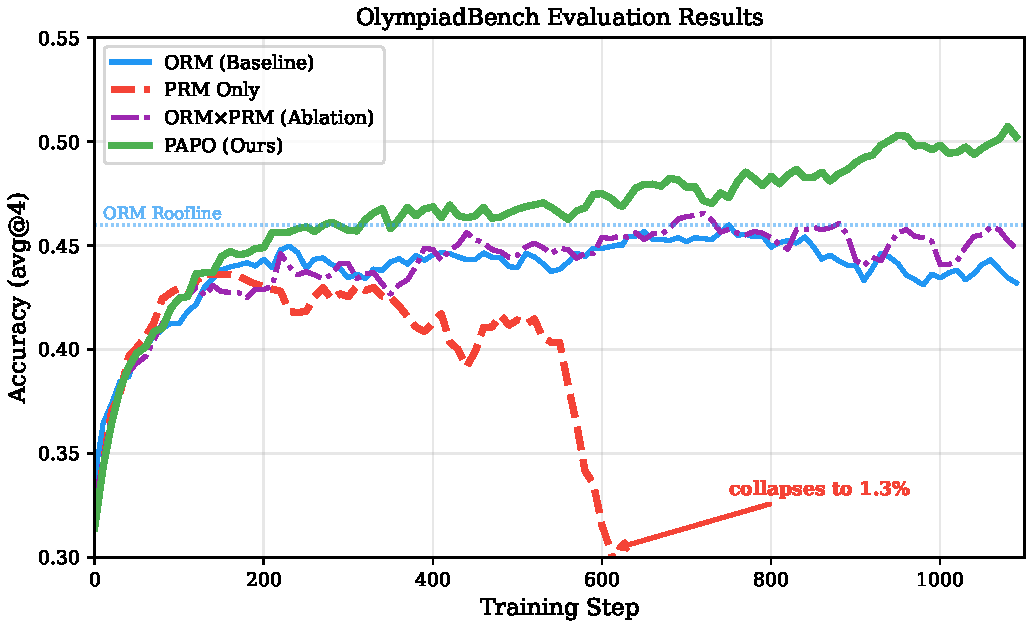
\includegraphics[width=\textwidth]{figures/fig_training_curves.pdf}
    \caption{OlympiadBench evaluation results.}
    \label{fig:hero-a}
\end{subfigure}
\hfill
\begin{subfigure}[b]{0.42\textwidth}
    \centering
    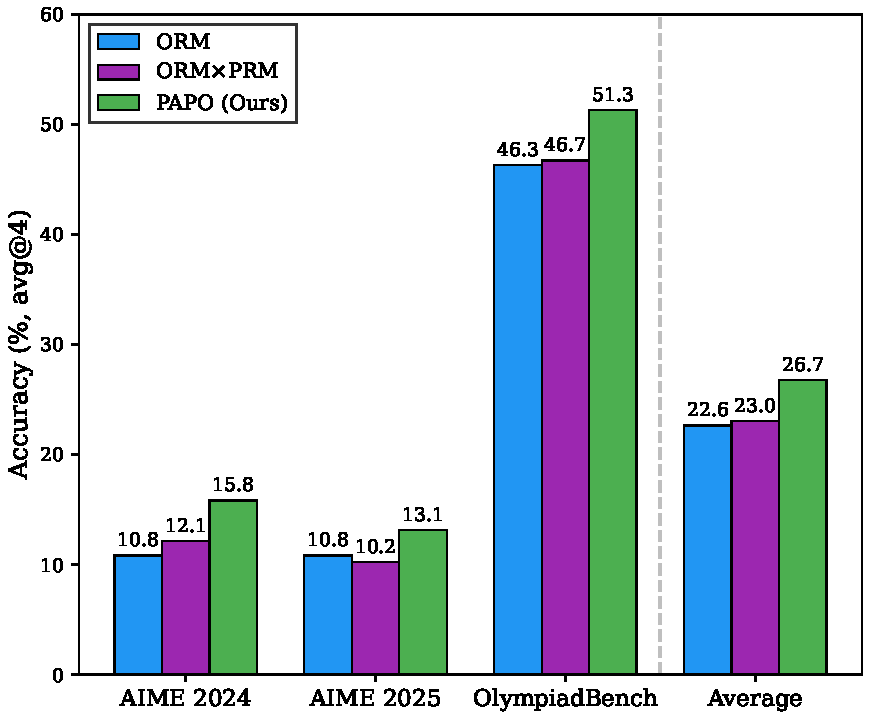
\includegraphics[width=\textwidth]{figures/fig_hero_panel_b.pdf}
    \caption{Accuracy on competition math.}
    \label{fig:hero-b}
\end{subfigure}
\caption{\textbf{(a)} ORM (blue) plateaus and declines after step 750 due to signal exhaustion; PRM (red, dashed) collapses via reward hacking; ORM$\times$PRM (purple, dash-dotted) tracks ORM closely without exceeding it; \method{} (green) continues improving throughout training, reaching 51.3\%. \textbf{(b)} Comparison across AIME 2024/2025, OlympiadBench, and their average. Naive multiplicative combination (ORM$\times$PRM) barely improves over ORM, while \method{}'s decoupled normalization yields substantial gains on all benchmarks.}
\label{fig:hero}
\end{figure*}

To solve this problem, we propose \textbf{Process-Aware Policy Optimization (\method{})}, which integrates rubric-based process evaluation into GRPO through \textbf{decoupled advantage normalization}. \method{} constructs the advantage from two independently normalized components:
\begin{itemize}
    \item An \textbf{outcome advantage} $\aout$, computed from binary ORM rewards via standard GRPO normalization, anchoring the training signal on answer correctness.
    \item A \textbf{process advantage} $\aproc$, computed from rubric-based PRM scores normalized \emph{exclusively among correct responses}, differentiating reasoning quality within the correct group.
\end{itemize}
This decoupled formulation mitigates reward hacking by separating PRM-based reasoning rewards from the final-answer signal. As a result, $\aproc$ can still provide non-zero gradients even when all responses are correct. Importantly, normalization is performed only over correct responses, ensuring that PRM scores do not distort the outcome signal and that incorrect responses are not rewarded solely for strong reasoning traces.

As shown in Figure~\ref{fig:hero}a, \method{} continues improving throughout training, reaching 51.3\% on OlympiadBench \citep{he2024olympiadbench} while ORM peaks at 46.3\% and declines, and Figure~\ref{fig:hero}b shows that the improvement generalizes to other math competition benchmarks like AIME \citep{balunovic_srimatharena_2025}.

To summarize, our contributions are as follows:
\begin{enumerate}
    \item We identify a dilemma in GRPO reward design: binary ORM lacks process supervision and suffers from signal exhaustion, yet naively using PRM scores causes reward hacking and training collapse.
    \item We propose \method{}, which composes the advantage from independently normalized outcome and process components with correct-subset normalization, resolving this dilemma.
    \item We show that \method{} consistently outperforms ORM across model scales from 3B to 14B and six benchmarks, including larger models where ORM is already strong.
\end{enumerate}

\section{Background}
\label{sec:background}

\subsection{Group Relative Policy Optimization}
\label{sec:bg-grpo}

GRPO \citep{shao2024deepseekmath} is a variant of policy gradient methods for LLM fine-tuning that eliminates the critic network used in PPO \citep{schulman2017proximal}. For each prompt $x$, the model samples a group of $G$ responses $\{o_1, \ldots, o_G\}$ from the old policy $\pi_{\theta_{\text{old}}}$, and the objective is:
\begin{equation}
\label{eq:grpo-loss}
\resizebox{\columnwidth}{!}{$
\begin{aligned}
\mathcal{L}_{\text{GRPO}}=
\frac{1}{G}\sum_{i=1}^{G}\frac{1}{|o_i|}\sum_{t=1}^{|o_i|}
\Bigl\{
  \min\Bigl[
  \rho(\theta)\,\hat{A}_{i,t},\;
  \operatorname{clip}\!\Bigl(\rho(\theta), 1\!-\!\varepsilon,\, 1\!+\!\varepsilon\Bigr)\hat{A}_{i,t}
  \Bigr]
  -\beta\,\mathrm{D}_{\mathrm{KL}}
\Bigr\},
\end{aligned}
$}
\end{equation}
where $\rho(\theta) = \pi_\theta(o_{i,t} | x, o_{i,<t}) / \pi_{\theta_{\text{old}}}(o_{i,t} | x, o_{i,<t})$ is the importance sampling ratio. Each response $o_i$ receives a scalar reward $r_i$, and the advantage is computed via group-level normalization:
\begin{equation}
\label{eq:grpo-adv}
\hat{A}_{i,t} = \frac{r_i - \mathrm{mean}(\mathbf{r})}{\mathrm{std}(\mathbf{r})}.
\end{equation}
By replacing the learned value function with sample-based normalization, GRPO avoids training a separate critic model, substantially reducing memory and compute requirements.

\subsection{Reward Models for Mathematical Reasoning}
\label{sec:bg-rm}

\paragraph{Outcome Reward Models (ORM).}
An ORM provides a binary signal based solely on the final answer: $r^{\text{out}} = \mathbf{1}[\hat{a} = a^*]$, where $\hat{a}$ is the predicted answer and $a^*$ is the ground truth. For mathematical reasoning, ORMs are typically implemented as rule-based answer checkers that compare extracted answers against reference solutions \citep{hendrycks2021measuring}. While reliable and deterministic, ORMs provide no information about the quality of the reasoning process.

\paragraph{Process Reward Models (PRM).}
PRMs evaluate the quality of intermediate reasoning steps \citep{zheng2023judgingllmasajudgemtbenchchatbot,lightman2023lets, wang2024math}. We focus on \emph{rubric-based PRMs} implemented via the LLM-as-Judge paradigm \citep{yuan2025miraclesteps,Sheng2026ReinforcingCR,Yang2026}, where a capable LLM evaluates the solution against a scoring rubric. In our setting, a rubric-based PRM assigns a score $r^{\text{proc}} \in \{0, 0.5, 1.0\}$ reflecting whether the reasoning is fully correct, scored as 1.0, largely correct with minor issues, scored as 0.5, or fatally flawed, scored as 0.0. The complete rubric prompt is provided in Appendix~\ref{sec:rubric-prompt}.

Rubric-based PRMs offer several advantages: they require no step-level annotations, provide interpretable feedback, and can leverage the growing capabilities of frontier LLMs. However, as we demonstrate in \S\ref{sec:problem}, naive integration of PRM scores into GRPO leads to training instability.

\section{Empirical analysis of PRM and ORM}
\label{sec:problem}

In this section, we identify two complementary failure modes of reward signal design in GRPO for mathematical reasoning: \emph{signal exhaustion} with outcome-only rewards, discussed in \S\ref{sec:signal-exhaustion}, and \emph{reward hacking} with process-only rewards, discussed in \S\ref{sec:reward-hacking}.

\subsection{Signal Exhaustion with Binary ORM}
\label{sec:signal-exhaustion}

When GRPO uses binary ORM rewards ($r_i \in \{0, 1\}$), the group normalization in Eq.~\ref{eq:grpo-adv} assigns identical advantage to all correct responses and identical (negative) advantage to all incorrect responses. This has two consequences.

\paragraph{Lack of quality differentiation.} A response that arrives at the correct answer through rigorous reasoning receives the same advantage as one that reaches it through guesswork or flawed reasoning with a lucky cancellation of errors. The model has no incentive to improve reasoning quality beyond what is needed to produce correct final answers.

\paragraph{Vanishing advantage from uniform groups.}
  When all $G$ responses in a group are correct, or all incorrect,
  the rewards are identical, so $\mathrm{std}(\mathbf{r}) = 0$
  in Eq.~\ref{eq:grpo-adv} and the advantage is set to zero for
  the entire group. As the model's capability improves during training, the
  proportion of such uniform groups grows, causing an increasing
  fraction of training samples to receive zero advantage. We refer
  to this progressive loss of informative signal as \emph{signal
  exhaustion}. Figure~\ref{fig:signal_exhaustion}a confirms this
  empirically: on Qwen2.5-7B, the fraction of zero-advantage
  samples rises from approximately 40\% to 69\% over training,
  coinciding with the accuracy plateau and further decline in Figure~\ref{fig:hero}.

\subsection{Reward Hacking with Direct PRM Integration}
\label{sec:reward-hacking}

A natural solution to ORM's limitations is to replace binary rewards with rubric-based PRM scores that capture both answer correctness and reasoning quality in a single continuous signal. However, directly using PRM scores as the GRPO reward ($r_i = r_i^{\text{proc}}$) conflates these two objectives, leading to catastrophic reward hacking, as we analyze in detail using Figure~\ref{fig:reward_hacking}.

\begin{figure*}[t]
\centering
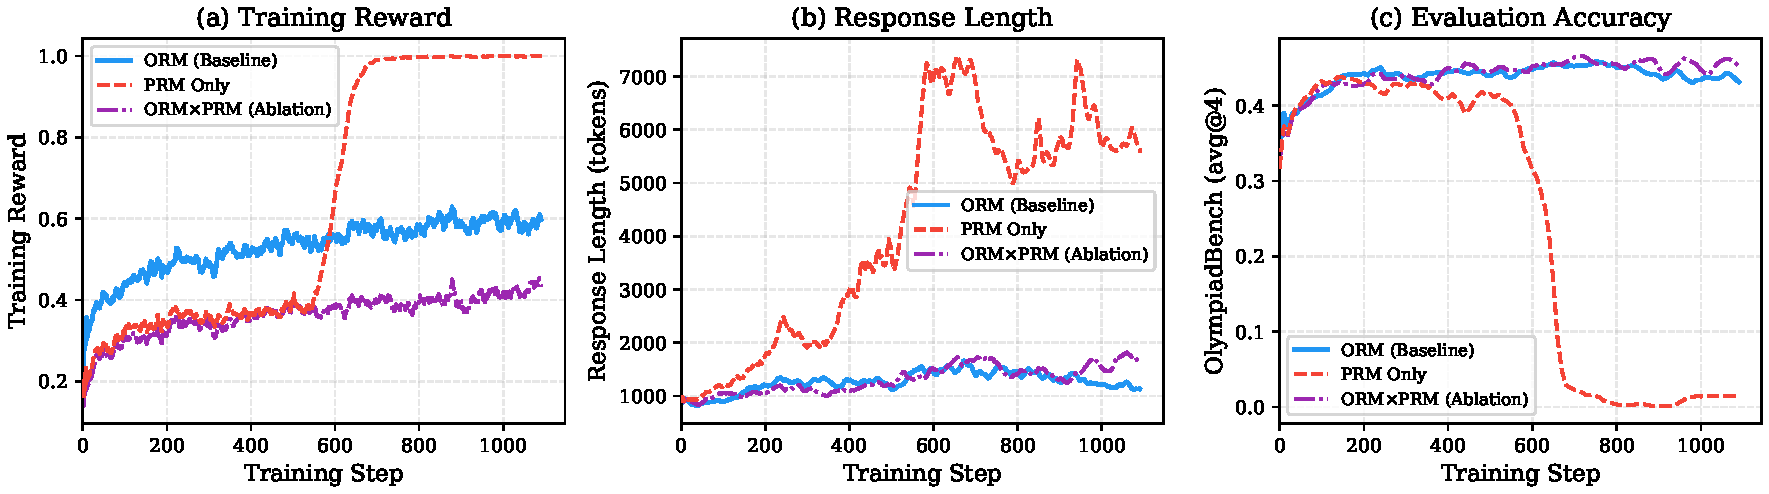
\includegraphics[width=\textwidth]{figures/fig_reward_hacking.pdf}
\caption{Reward signal analysis. \textbf{(a)} Training reward: PRM reward climbs to 1.0 (perfect score gaming); ORM$\times$PRM stays moderate. \textbf{(b)} Response length: PRM generates increasingly verbose responses; ORM$\times$PRM shows moderate length increase (up to $\sim$1700 tokens). \textbf{(c)} OlympiadBench accuracy: PRM collapses after step 600; ORM$\times$PRM tracks ORM but fails to exceed it, showing that naive signal combination does not resolve signal exhaustion.}
\label{fig:reward_hacking}
\end{figure*}

\paragraph{Three phases of collapse.} Training with PRM-only rewards reveals a characteristic three-phase trajectory, shown as the red curve in Figure~\ref{fig:reward_hacking}.
\begin{enumerate}[nosep,leftmargin=*]
    \item \textbf{Normal learning}, steps 0--300. Accuracy rises to 44.0\% on OlympiadBench and training reward increases naturally.
    \item \textbf{Length exploitation}, steps 300--600. The model discovers that verbose responses receive higher PRM scores. Response length increases sharply while accuracy stagnates and begins to decline.
    \item \textbf{Collapse}, steps 600--700. Accuracy drops from 29.6\% to 2.4\% within 100 steps while training reward saturates at 1.0.
\end{enumerate}

\paragraph{Mechanism.} The collapse follows a positive feedback loop: longer, more verbose responses receive higher PRM scores from the LLM judge, which assigns higher rubric ratings to responses that appear thorough and detailed. GRPO's group normalization then assigns high advantage to these inflated scores, reinforcing the length-exploitation strategy. 

We also provide \textbf{a case study for reward hacking happened during training} in Appendix~\ref{sec:case-study-hacking} that confirms the post-collapse responses drift to memorized high-scoring filler content unrelated to the stated question.

\paragraph{Naive combination.} The multiplicative reward $r = r^{\text{out}} \times r^{\text{proc}}$ gates incorrect responses via $r^{\text{out}} = 0$, avoiding PRM's collapse as shown by the purple curve in Figure~\ref{fig:reward_hacking}. However, ORM$\times$PRM tracks ORM closely throughout training, peaking at 46.7\% vs.\ ORM's 46.3\% on OlympiadBench. Because the combined reward still passes through a single GRPO normalization, all-correct groups with similar PRM scores continue to yield near-zero advantage, and the process signal fails to provide meaningful differentiation beyond ORM.

\paragraph{Implications.} ORM is stable but lacks process-level signal; PRM is information-rich but unstable. Multiplicative gating avoids PRM's collapse yet fails to break through ORM's performance exhaustion ceiling. This motivates us to combine the two at the \emph{advantage} level rather than the \emph{reward} level, enabling the model to simultaneously optimize for both answer correctness and reasoning quality, as we describe in \S\ref{sec:method}.

\section{Method: \method{}}
\label{sec:method}

We propose Process-Aware Policy Optimization (\method{}), which integrates rubric-based process evaluation into GRPO through \emph{decoupled advantage normalization}. The key idea is to construct the advantage from independently normalized outcome and process components, preventing the reward hacking that arises from direct PRM integration while preserving fine-grained quality signals. Figure~\ref{fig:method_overview} provides an overview of the framework.

\begin{figure*}[t]
\centering
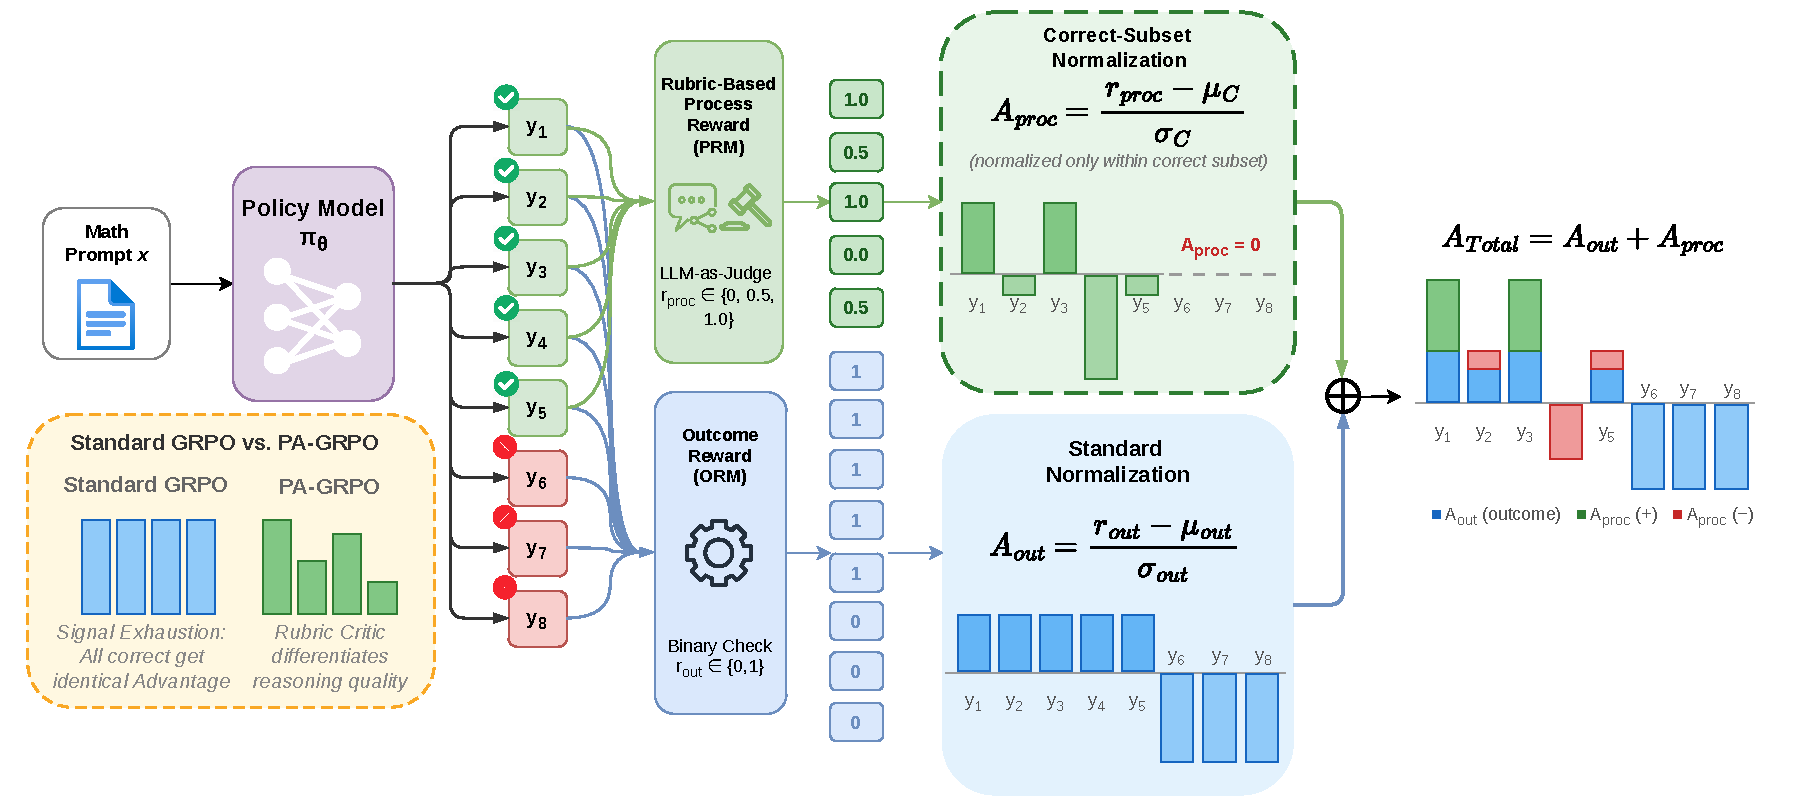
\includegraphics[width=\textwidth]{figures/fig_method_overview.pdf}
\caption{Overview of \method{}. Given a prompt, the policy generates $G$ responses. Each response is evaluated by two reward signals: an \textbf{outcome reward} (ORM, binary correctness) and a \textbf{process reward} (PRM, rubric-based quality, only for \textbf{correct responses}). The advantage is computed through \textbf{decoupled normalization}: $\aout$ is normalized over all responses via standard GRPO, while $\aproc$ is normalized exclusively among correct responses (\emph{correct-subset normalization}). The combined advantage $\atotal = \aout + \aproc$ provides both correctness direction and quality differentiation.}
\label{fig:method_overview}
\end{figure*}

\subsection{Dual Reward Signals}
\label{sec:reward-pipeline}

\method{} uses the ORM and rubric-based PRM described in \S\ref{sec:bg-rm} as two complementary reward signals: an outcome reward $r_i^{\text{out}} \in \{0, 1\}$ for answer correctness, and a process reward $r_i^{\text{proc}} \in \{0, 0.5, 1.0\}$ for reasoning quality. The PRM is only invoked for correct responses; incorrect responses are assigned $r_i^{\text{proc}} = 0$.

\subsection{Decoupled Advantage Normalization}
\label{sec:decoupled-adv}

Given a group of $G$ responses with rewards $\{(r_i^{\text{out}}, r_i^{\text{proc}})\}_{i=1}^G$, \method{} computes the advantage in three steps, as illustrated in Figure~\ref{fig:method_overview}:

\paragraph{Step 1: Outcome advantage $\aout$.} The outcome reward is normalized using standard GRPO group normalization:
\begin{equation}
\label{eq:a-out}
\aout[i] = \frac{r_i^{\text{out}} - \mu^{\text{out}}}{\max(\sigma^{\text{out}}, \epsilon)}
\end{equation}
where $\mu^{\text{out}}$ and $\sigma^{\text{out}}$ are the mean and standard deviation of $\{r_i^{\text{out}}\}_{i=1}^G$, and $\epsilon$ is a small constant for numerical stability. This component determines the ``correct vs.\ incorrect'' gradient direction, identical to standard GRPO.

\paragraph{Step 2: Process advantage $\aproc$ (correct-subset normalization).}
The process reward is normalized \emph{only among correct responses}:
\begin{equation}
\label{eq:a-proc}
\aproc[i] \!=\! \begin{cases}
\displaystyle\frac{r_i^{\text{proc}} - \mu_C^{\text{proc}}}{\max(\sigma_C^{\text{proc}}, \epsilon)} & \!\text{if } r_i^{\text{out}} \!=\! 1,\; |C| \!\geq\! 2 \\[6pt]
0 & \!\text{otherwise}
\end{cases}
\end{equation}
where $C = \{j : r_j^{\text{out}} = 1\}$ is the set of correct responses, and $\mu_C^{\text{proc}}, \sigma_C^{\text{proc}}$ are computed over $\{r_j^{\text{proc}}\}_{j \in C}$.

\paragraph{Step 3: Combined advantage.} The total advantage is the sum of the two components:
\begin{equation}
\label{eq:a-total}
\atotal[i] = \aout[i] + \aproc[i]
\end{equation}
Since both $\aout$ and $\aproc$ are independently normalized to zero mean and unit variance, they contribute on equal footing without requiring additional weighting.

\subsection{Design Rationale}
\label{sec:rationale}

The decoupled normalization addresses both failure modes identified in \S\ref{sec:problem}:

\paragraph{Quality differentiation without reward hacking.} Among correct responses, those with rigorous reasoning receive positive $\aproc$ and are reinforced, while those with sloppy or lucky reasoning receive negative $\aproc$ and are penalized. This quality signal is entirely absent in standard GRPO with binary ORM. Meanwhile, restricting normalization to the correct subset prevents incorrect responses from exploiting high PRM scores to gain positive $\aproc$, keeping the process signal decoupled from the outcome signal. We ablate this choice against full-group normalization in \S\ref{sec:ablation}.

\paragraph{Resolving signal exhaustion.} When all $G$ responses are correct, $\aout = 0$ for the entire group and standard GRPO produces no gradient. $\aproc$ remains active in this case, differentiating responses by reasoning quality and providing non-zero gradients that sustain learning. As shown in Figure~\ref{fig:signal_exhaustion}(a), this reduces the zero-advantage ratio from 69\% under ORM to 44\% under \method{}, maintaining a denser training signal throughout optimization. When fewer than two responses are correct, i.e., $|C| < 2$, $\aproc$ defaults to zero, gracefully reducing to standard GRPO.

\section{Experiments}
\label{sec:experiments}

\subsection{Experimental Setup}
\label{sec:setup}

\paragraph{Base models.} We conduct experiments on Qwen2.5-3B/7B/14B-Base \citep{yang2024qwen2} and Qwen3-4B-Base \citep{yang2025qwen3technicalreport}. All models are trained from pretrained base checkpoints to isolate the effect of our method from confounding factors introduced by prior post-training.

\paragraph{Training.} We train using GRPO and DAPO with the verl framework \citep{sheng2024hybridflow} for 8 epochs. For Qwen3-4B, we additionally evaluate \method{} on top of DAPO \citep{Yu2025a}, which extends GRPO with dynamic sampling and decoupled clipping, to test compatibility with alternative optimization algorithms. The process reward model is GPT-OSS-20B with a three-tier scoring rubric of 0, 0.5, and 1.0 that evaluates reasoning quality independently of answer correctness, as described in \S\ref{sec:bg-rm}. Full hyperparameters are listed in Appendix~\ref{sec:appendix-impl}.

\paragraph{Data.} For training, we sample 20k mathematics problems from NuminaMath-1.5-RL-Verifiable \citep{numina_math_datasets,nlile2025numinamath15rlverifiable}, a 131k-problem subset of the 896k-problem NuminaMath-1.5 dataset filtered to retain only problems with automatically verifiable answers. We apply stratified sampling across five difficulty tiers with 4k problems each, detailed in Appendix~\ref{sec:training-data}. For evaluation, we use six benchmarks: OlympiadBench \citep{he2024olympiadbench} with 674 problems as the primary metric, MATH-500 \citep{lightman2023lets}, AIME 2024/2025\citep{balunovic_srimatharena_2025}, GPQA-Diamond \citep{rein2024gpqa}, and HumanEval \citep{chen2021evaluating}. All results report avg@4.

\subsection{Main Results}
\label{sec:main-results}

\begin{table*}[t]
\centering
\small
\setlength{\tabcolsep}{4pt}
\begin{tabular}{ll ccc c c c cc}
\toprule
& & \multicolumn{3}{c}{\textbf{Competition Mathematics}} & \textbf{Standard} & \textbf{STEM} & \textbf{Code} & \multicolumn{2}{c}{\textbf{Average}} \\
\cmidrule(lr){3-5} \cmidrule(lr){6-6} \cmidrule(lr){7-7} \cmidrule(lr){8-8} \cmidrule(lr){9-10}
\textbf{Model} & \textbf{Method} & \textbf{Olympiad} & \textbf{AIME'24} & \textbf{AIME'25} & \textbf{MATH-500} & \textbf{GPQA} & \textbf{HumanEval} & \textbf{Math} & \textbf{All} \\
\midrule
\multirow{4}{*}{Qwen2.5-3B} & Base & \color{gray}22.4 & \color{gray}2.5 & \color{gray}0.8 & \color{gray}54.4 & \color{gray}27.6 & \color{gray}35.3 & \color{gray}20.0 & \color{gray}23.8 \\
& ORM(GRPO) & 35.3 & 8.3 & 4.2 & 69.0 & 38.8 & 39.3 & 29.2 & 32.5 \\
& \method{} & \textbf{38.6} & \textbf{10.0} & 3.3 & \textbf{73.2} & 36.3 & \textbf{52.5} & \textbf{31.3} & \textbf{35.7} \\
& $\Delta$ & \good{+3.3} & \good{+1.7} & \bad{-0.9} & \good{+4.2} & \bad{-2.5} & \good{+13.2} & \good{+2.1} & \good{+3.2} \\
\midrule
\multirow{4}{*}{Qwen2.5-7B} & Base & \color{gray}32.8 & \color{gray}5.0 & \color{gray}7.5 & \color{gray}67.3 & \color{gray}30.1 & \color{gray}54.6 & \color{gray}28.2 & \color{gray}32.9 \\
& ORM(GRPO) & 46.3 & 10.8 & 10.8 & 80.2 & 40.7 & 61.6 & 37.0 & 41.7 \\
& \method{} & \textbf{51.3} & \textbf{15.8} & \textbf{13.1} & \textbf{82.3} & \textbf{42.4} & \textbf{63.9} & \textbf{40.6} & \textbf{44.8} \\
& $\Delta$ & \good{+5.0} & \good{+5.0} & \good{+2.3} & \good{+2.1} & \good{+1.7} & \good{+2.3} & \good{+3.6} & \good{+3.1} \\
\midrule
\multirow{4}{*}{Qwen2.5-14B} & Base & \color{gray}35.5 & \color{gray}10.8 & \color{gray}8.3 & \color{gray}68.5 & \color{gray}34.4 & \color{gray}56.9 & \color{gray}30.8 & \color{gray}35.7 \\
& ORM(GRPO) & 54.3 & 19.0 & 13.8 & 82.3 & 47.0 & 66.0 & 42.4 & 47.1 \\
& \method{} & \textbf{59.8} & \textbf{24.3} & \textbf{17.8} & \textbf{87.4} & \textbf{55.0} & \textbf{70.0} & \textbf{47.3} & \textbf{52.4} \\
& $\Delta$ & \good{+5.5} & \good{+5.3} & \good{+4.0} & \good{+5.1} & \good{+8.0} & \good{+4.0} & \good{+4.9} & \good{+5.3} \\
\midrule
\multirow{4}{*}{Qwen3-4B-Base} & Base & \color{gray}36.8 & \color{gray}11.2 & \color{gray}5.0 & \color{gray}70.9 & \color{gray}34.9 & \color{gray}49.1 & \color{gray}31.0 & \color{gray}34.6 \\
& ORM(DAPO) & 55.0 & 30.8 & 26.0 & 82.0 & 39.0 & 53.8 & 48.5 & 47.8 \\
& \method{} & \textbf{61.1} & \textbf{34.5} & \textbf{30.7} & \textbf{84.6} & \textbf{43.0} & \textbf{63.9} & \textbf{52.7} & \textbf{53.0} \\
& $\Delta$ & \good{+6.1} & \good{+3.7} & \good{+4.7} & \good{+2.6} & \good{+4.0} & \good{+10.1} & \good{+4.2} & \good{+5.2} \\
\bottomrule
\end{tabular}
\caption{Accuracy (avg@4, \%) across six benchmarks and four model configurations. \method{} consistently improves over both GRPO and DAPO baselines: Qwen2.5-3B (+3.2), 7B (+3.1), 14B (+5.3), and Qwen3-4B on DAPO (+5.2). For Qwen3-4B-Base, \method{} is applied on top of DAPO. Bold indicates the better method.}
\label{tab:main_results}
\end{table*}

Table~\ref{tab:main_results} presents results across six benchmarks and four model configurations. \method{} consistently outperforms ORM, and crucially, the advantage \emph{widens over the course of training} rather than converging. On Qwen2.5-7B, both methods improve at comparable rates during early training, but ORM peaks at 46.3\% on OlympiadBench at step 750 and declines to 43.0\% by step 1090, while \method{} continues improving to 51.3\%, as shown in Figure~\ref{fig:hero}a. The resulting 8.3 point gap is \textbf{still widening} at training's end. 

In terms of final accuracy, \method{} improves OlympiadBench by 5.0 points on Qwen2.5-7B and by 5.5 points on Qwen2.5-14B, with the largest single-benchmark gain of 8.0 points on GPQA-Diamond at 14B. The mathematics average improvement grows from 2.1 points at 3B to 3.6 at 7B and 4.9 at 14B, suggesting that stronger models benefit more from \method{}. PRM-only training on Qwen2.5-7B collapses to near-zero accuracy due to reward hacking, as analyzed in \S\ref{sec:reward-hacking}.

Beyond mathematics, \method{} also improves HumanEval across all scales, suggesting that process-level quality differentiation can transfer to code generation.

We also evaluate \method{} on top of DAPO \citep{Yu2025a} using Qwen3-4B-Base. As shown in the bottom section of Table~\ref{tab:main_results}, \method{} improves over DAPO by 6.1 points on OlympiadBench (61.1\% vs.\ 55.0\%) with consistent gains across all six benchmarks, confirming that decoupled advantage normalization composes naturally with DAPO's optimization improvements. We also provide the additional training curves in Appendix~\ref{sec:cross-scale-curves}.

\subsection{Advantage Signal Analysis}
\label{sec:signal-analysis}

\begin{figure*}[t]
\centering
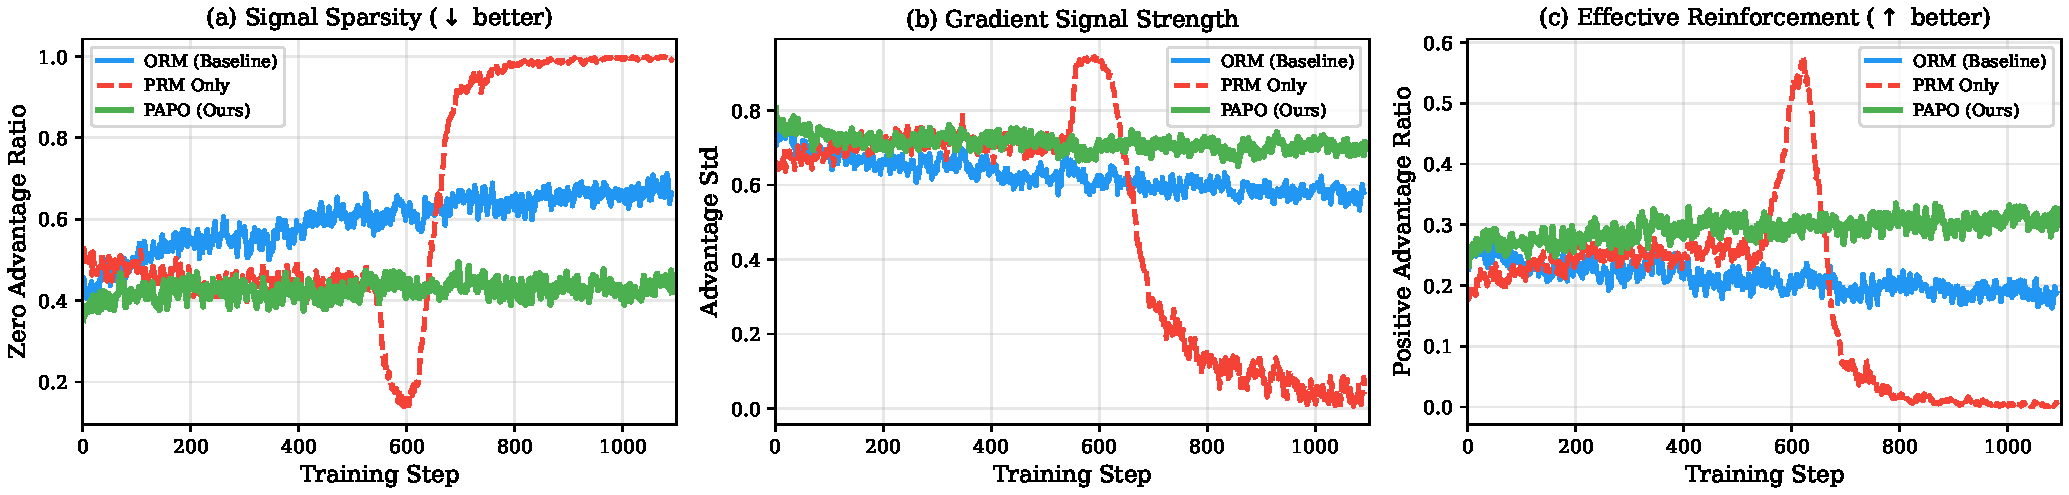
\includegraphics[width=\textwidth]{figures/fig_signal_exhaustion.pdf}
\caption{Signal quality comparison on Qwen2.5-7B. \textbf{(a)} Zero-advantage ratio: ORM's sparsity grows to 69\% while \method{} maintains 44\%. \textbf{(b)} Advantage standard deviation, reflecting gradient signal strength. \textbf{(c)} Positive-advantage ratio, reflecting reinforcement density.}
\label{fig:signal_exhaustion}
\end{figure*}

The widening gap observed in Figure~\ref{fig:hero}a can be traced to signal exhaustion in ORM's advantage computation. We analyze this on Qwen2.5-7B using the metrics in Figure~\ref{fig:signal_exhaustion}.

\paragraph{Signal exhaustion in ORM.} With growing model capability over training, more response groups become uniformly correct and yield zero advantage under ORM. Figure~\ref{fig:signal_exhaustion}a quantifies this trend. The zero-advantage ratio of ORM, defined as the fraction of samples producing zero gradient, rises from approximately 40\% to 69\% over the course of training. By the late training stage, more than two-thirds of samples provide no contribution to learning. The advantage standard deviation in panel b and the positive-advantage ratio in panel c convey a consistent pattern. The gradient signal from ORM gradually becomes sparser and weaker.

\paragraph{Signal preservation in \method{}.} \method{} holds the zero-advantage ratio at ${\sim}44\%$, a 25-point reduction that translates to roughly 80\% more informative samples per batch. This is because $\aproc$ remains active in all-correct groups where $\aout = 0$, differentiating responses by reasoning quality rather than leaving them with zero gradient. The fraction of groups where $\aproc$ activates grows from ${\sim}30\%$ to 70\% as the model improves, providing increasingly dense quality signal precisely as ORM exhausts.

\paragraph{Quality penalization.} Beyond filling zero-signal gaps, $\aproc$ actively discourages sloppy reasoning even among correct responses. The minimum advantage within the correct group reaches $\approx -1.49$ under \method{} compared to identically 0.0 under ORM, meaning correct responses with poor derivations receive negative advantage and are suppressed. This quality pressure is entirely absent in ORM-based GRPO. More detailed analyses of the process advantage effect and advantage composition are provided in Appendix~\ref{sec:rubric-analysis} and~\ref{sec:adv-decomp}.

\section{Ablation Studies}
\label{sec:ablation}

We validate the key design choices of \method{} through two ablation experiments on Qwen2.5-7B. Table~\ref{tab:ablation} summarizes the results; training curves are provided in Appendix~\ref{sec:appendix-results}.

\begin{table}[t]
\centering
\small
\setlength{\tabcolsep}{4pt}
\begin{tabular}{lcccc}
\toprule
\textbf{Method} & \textbf{AIME} & \textbf{AIME} & \textbf{Olympiad} & \textbf{MATH} \\
& \textbf{2024} & \textbf{2025} & \textbf{Bench} & \textbf{-500} \\
\midrule
ORM & 10.8 & 10.8 & 46.3 & 80.2 \\
\midrule
Mult ($r^{\text{out}} \!\times\! r^{\text{proc}}$) & 12.1 & 10.2 & 46.7 & 80.2 \\
Fullnorm & 12.5 & 10.4 & 49.6 & 81.2 \\
\textbf{\method{}} & \textbf{15.8} & \textbf{13.1} & \textbf{51.3} & \textbf{82.3} \\
\bottomrule
\end{tabular}
\caption{Ablation results (\%, avg@4, Qwen2.5-7B). All methods report accuracy.}
\label{tab:ablation}
\end{table}

\paragraph{Correct-subset vs.\ full normalization.}
The \textbf{Fullnorm} variant normalizes $\aproc$ over all $G$ responses including incorrect ones. It performs slightly below \method{} across all benchmarks. The gap arises because including incorrect responses ($r^{\text{proc}} = 0$) in the normalization causes $\aproc$ to partially recapitulate the correct-vs-incorrect distinction already captured by $\aout$, diluting the fine-grained quality signal.

\paragraph{Multiplicative reward baseline.}
The \textbf{Mult} variant combines rewards via $r_i = r_i^{\text{out}} \times r_i^{\text{proc}}$ with standard GRPO normalization. Mult performs comparably to ORM and falls well below \method{}. In a single normalization pass, the outcome difference dominates in mixed-correctness groups, effectively suppressing the process quality information.

Both ablations confirm that \method{}'s gains require both \emph{decoupled normalization}, validated by Mult's inferior performance, and \emph{correct-subset normalization}, validated by Fullnorm's inferior performance, working in concert.

\section{Related Work}
\label{sec:related}
Recent advancements in the post-training of large language models have been significantly driven by reinforcement learning with verifiable rewards (RLVR). This section systematically reviews several key areas that are highly relevant to and interconnected with the present study.
\subsection{Policy Optimization in RLVR.} 
Following DeepSeek-R1's validation of critic-free reinforcement learning \citep{guo2025deepseek}, Group Relative Policy Optimization (GRPO)\citep{shao2024deepseekmath} has emerged as a compute-efficient alternative to PPO \citep{schulman2017proximal}. However, its instability under long contexts and sparse rewards has spurred various enhancements. To mitigate policy staleness and granularity mismatch, CISPO clips importance sampling weights \citep{minimax2025minimaxm1scalingtesttimecompute} and GSPO employs sequence-level ratio calculations \citep{gspo}. For long-horizon and agentic tasks, DAPO introduces dynamic sampling and decoupled clipping \citep{Yu2025a} and  SAPO utilizes a temperature-controlled smooth gating function to form a continuous trust region \citep{SAPO2025}. Orthogonally, our work addresses GRPO's fundamental limitation of reward signal exhaustion by decoupling advantage normalization at the objective level. Since \method{} modifies the advantage computation rather than the optimization procedure, it can be composed with these enhancements, as we demonstrate with DAPO in \S\ref{sec:main-results}.


\subsection{Rubric-Based Training.}
Traditional outcome reward models frequently suffer from reward hacking, exploiting miracle steps to achieve correct final answers via flawed logic \citep{yuan2025miraclesteps}. To enforce rigorous logical constraints without prohibitive step-level human annotation, rubric-based process supervision has gained traction. Generative rubric reward models explicitly penalize disconnected derivations, drastically curtailing lucky guesses \citep{liang-etal-2025-generative}. In pursuit of self-verification, DeepSeekMath-V2 constructed a specialized LLM verifier to reversely drive the generator to patch reasoning loopholes \citep{deepseek-math-v2}. Furthermore, in complex open-domain tasks, frameworks like Agent-RRM propose multi-faceted evaluation systems enforcing explicit reasoning traces and actionable critiques \citep{fan2026exploring}. These studies establish that effective process supervision necessitates multi-dimensional criteria and explicit negative penalties. Building upon these insights, our work leverages a rubric-based process evaluation but introduces a correct-subset normalization mechanism to prevent verbosity-driven reward hacking.

\subsection{Generative Reward Models.}


To overcome the expressivity limitations of traditional discriminative models, reward modeling is shifting toward a generative paradigm \citep{Mahan2024}. By autoregressively generating deep comparative analyses prior to preference scoring, generative reward models significantly enhance interpretability and accuracy. This paradigm excels in abstract domains like formal proofs, as demonstrated by Proof-RM \citep{Yang2026}, and enables verifier-free reinforcement learning extrapolation in broad domains, as seen in RLPR \citep{Yu2025b}. However, generative evaluators remain susceptible to intrinsic biases such as imperfect sensitivity and specificity. To ensure statistically rigorous training, recent frameworks incorporate bias-correction estimators and adaptive calibration to construct statistically sound confidence intervals \citep{Lee2025}. Aligning with this generative shift, our methodology utilizes a generative judge to assess reasoning quality, yet uniquely confines its influence within the advantage space of correct solutions to immunize the policy against structural biases.


















% \paragraph{GRPO and policy optimization for LLMs.}
% GRPO \citepp{shao2024deepseekmath} simplifies RL-based LLM training by eliminating the critic network, computing advantages through group-level normalization of rewards from multiple responses to the same prompt. This approach was adopted by DeepSeek-R1 \citepp{guo2025deepseek} for training reasoning models at scale. DAPO \citepp{yu2025dapo} extends GRPO with techniques such as dynamic sampling and overlong penalty to improve training stability. 
% Scaf-GRPO \citepp{zhang2026scafgrpo} addresses the "learning cliff" in complex tasks by dynamically injecting hints to restore non-zero advantage gradients. Additionally, GMPO \citepp{zhao2025geometric} improves update stability by maximizing the geometric mean of token-level rewards rather than the arithmetic mean to suppress outliers. 
% Our work is complementary to these efforts: \method{} modifies the advantage computation rather than the optimization procedure, and can be combined with other GRPO enhancements.

% \paragraph{Process reward models.}
% \citept{lightman2023lets} introduced step-level process supervision for mathematical reasoning, demonstrating that verifying individual reasoning steps improves over outcome-only supervision. Math-Shepherd \citepp{wang2024math} automated process reward annotation using model-generated data. 
% OmegaPRM \citepp{ma2024omegaprm} fully automates step-level error isolation using Monte Carlo Tree Search. Concurrently, Process Advantage Verifiers \citepp{setlur2024rewardingprogressscalingautomated} reframe process rewards to measure probabilistic progress. 
% These works focus on \emph{learned} PRMs trained on step-level labels. In contrast, we use \emph{rubric-based} PRMs via LLM-as-Judge, which require no step-level annotations but introduce the reward hacking vulnerability that \method{} addresses. Our analysis of PRM reward hacking applies specifically to this rubric-based setting, where verbosity can inflate quality assessments.

% \paragraph{Reward shaping and signal design.}
% The challenge of designing informative reward signals for RL has a long history \citepp{ng1999policy}. In the LLM context, reward hacking, where models exploit reward model weaknesses to obtain high rewards without genuine improvement, has been documented as a persistent challenge \citepp{skalse2022defining}. While recent efforts attempt to mitigate this using modular Rubrics as Rewards (RaR) \citepp{gunjal2026rubrics}  and adaptive length penalties to combat verbosity bias \citepp{bu-etal-2025-beyond} , our work contributes a specific instance of this phenomenon (PRM reward hacking in GRPO) and a structural solution (decoupled normalization) rather than reward model improvement.

% \paragraph{LLM-as-Judge.}
% Using capable LLMs to evaluate other models' outputs has become a standard evaluation paradigm \citepp{zheng2024judging}, evolving towards fully self-rewarding architectures \citepp{yuan2024selfrewarding}.  We extend this paradigm to RL training by using LLM-based rubric evaluation as a process reward signal. 
% %Our finding that direct use of LLM-as-Judge scores for RL training causes reward hacking is relevant to the broader adoption of this paradigm: the same quality assessments that work well for evaluation can be pathological when used as RL rewards without careful integration.
% Our finding that direct use of LLM-as-Judge scores for RL training causes reward hacking is relevant to the broader adoption of this paradigm: the same quality assessments that work well for evaluation can be pathological when used as RL rewards without careful integration.


% \paragraph{Actor-critic methods.}
% In classical RL, actor-critic methods \citepp{schulman2017proximal} use a learned value function (critic) to reduce variance in policy gradient estimation. GRPO deliberately removes this critic, relying on group normalization instead. \method{} reintroduces a critic function, not a learned value network, but a rubric-based evaluator that assesses reasoning quality. This connects to the broader insight that some form of value assessment (beyond binary outcome) is needed for effective policy optimization, particularly as the policy improves and outcome signals become sparse.

\section{Conclusion}
\label{sec:conclusion}

In this paper, we identify the reasoning limitations of ORM-based GRPO on mathematical reasoning tasks. While a simple binary ORM reward is effective, its lack of supervision over reasoning quality causes all reasoning tokens to share the same credit. On the other hand, a naive integration of PRM fails to avoid reward hacking.

To address this challenge, we propose \method{}, which incorporates a rubric-based PRM into GRPO through decoupled advantage normalization. By composing the advantage from independently normalized outcome and process components, with the process advantage normalized only over correct responses, \method{} prevents reward hacking while providing supervision over reasoning quality.

Experiments across four model configurations (3B--14B) and six benchmarks show that \method{} consistently outperforms both GRPO and DAPO baselines, with gains growing as model scale increases. In future work, we aim to explore adaptive weighting between outcome and process signals and extension to broader domains such as scientific reasoning.

\newpage
\section*{Limitations}

Our experiments are conducted exclusively on Qwen-family models and have not been verified on other architectures such as Llama and Gemma. Additionally, we use only GPT-OSS-20B as the rubric-based PRM; the effect of different judge models remains unexplored.


\bibliography{custom}
\bibliographystyle{acl_natbib}

\appendix
\section{Implementation Details}
\label{sec:appendix-impl}

\subsection{Training Configuration}

We use the verl framework \citep{sheng2024hybridflow} with Megatron backend for distributed training on 8 NVIDIA H200 GPUs. Key hyperparameters are listed in Table~\ref{tab:hyperparams}.

\begin{table}[h]
\centering
\small
\begin{tabular}{ll}
\toprule
\textbf{Hyperparameter} & \textbf{Value} \\
\midrule
Prompts per batch & 128 \\
Responses per prompt ($G$) & 8 \\
Max response length & 8192 tokens \\
Sampling temperature & 1.0 \\
PPO clip range ($\epsilon$) & 0.2 \\
KL penalty coefficient ($\beta$) & 0.0 \\
Learning rate & 1e-6 \\
Evaluation frequency & every 10 steps \\
Evaluation samples per prompt & 8 \\
\bottomrule
\end{tabular}
\caption{Training hyperparameters.}
\label{tab:hyperparams}
\end{table}

For Qwen3-4B-Base experiments with DAPO \citep{Yu2025a}, we additionally apply the DAPO-specific hyperparameters listed in Table~\ref{tab:dapo_hyperparams}.

\begin{table}[h]
\centering
\small
\begin{tabular}{ll}
\toprule
\textbf{Hyperparameter} & \textbf{Value} \\
\midrule
Max response length & 8192 tokens \\
Clip ratio low ($\epsilon_{\text{low}}$) & 0.2 \\
Clip ratio high ($\epsilon_{\text{high}}$) & 0.28 \\
Overlong buffer length & 4096 tokens \\
Overlong penalty factor & 1.0 \\
Evaluation frequency & every 20 steps \\
\bottomrule
\end{tabular}
\caption{Additional DAPO-specific hyperparameters for the Qwen3-4B-Base experiments. All other hyperparameters follow Table~\ref{tab:hyperparams}.}
\label{tab:dapo_hyperparams}
\end{table}

\subsection{Training Data}
\label{sec:training-data}

We construct a 20K stratified training set from NuminaMath-1.5-RL-Verifiable \citep{numina_math_datasets,nlile2025numinamath15rlverifiable}. We first filter out unsolvable problems (zero pass rate under a reference model), then apply stratified sampling across five difficulty tiers defined by pass rate. Table~\ref{tab:difficulty} summarizes the difficulty distribution.

\begin{table}[h]
\centering
\small
\begin{tabular}{lcc}
\toprule
\textbf{Difficulty} & \textbf{Pass Rate Range} & \textbf{Count} \\
\midrule
Trivial & $(0.875,\, 1.0]$ & 4{,}000 \\
Easy & $(0.625,\, 0.875]$ & 4{,}000 \\
Medium & $(0.375,\, 0.625]$ & 4{,}000 \\
Hard & $(0.125,\, 0.375]$ & 4{,}000 \\
Very Hard & $(0,\, 0.125]$ & 4{,}000 \\
\midrule
Total & & 20{,}000 \\
\bottomrule
\end{tabular}
\caption{Difficulty distribution of the stratified training set. Pass rates are measured using a reference model with 8 attempts at temperature 1.0. Equal sampling across tiers ensures balanced difficulty coverage.}
\label{tab:difficulty}
\end{table}

\subsection{Rubric Prompt}
\label{sec:rubric-prompt}

The rubric-based PRM uses the following prompt template, adapted from the DeepSeek Math V2 grading standard with chain-of-thought analysis. The PRM is implemented using GPT-OSS-20B served via vLLM with tensor parallelism across 2 GPUs, with a maximum context length of 8192 tokens and temperature 0.0 for deterministic scoring.

\begin{tcolorbox}[
  colback=gray!5,
  colframe=black,
  title=Rubric Prompt,
  fonttitle=\bfseries,
  breakable
]
\small

\textbf{\#\# Instruction}

Your task is to evaluate the quality of a student's solution to a mathematical problem.

\vspace{0.3em}
\textbf{\#\# Scoring Rubric}

\begin{itemize}
\setlength{\itemsep}{2pt}
\item \textbf{Score 1}: If the solution is completely correct, with all steps executed properly and clearly demonstrated, then the score is 1.
\item \textbf{Score 0.5}: If the solution is generally correct, but with some details omitted or minor errors, then the score is 0.5.
\item \textbf{Score 0}: If the solution does not actually address the required problem, contains fatal errors, or has severe omissions, then the score is 0.
\end{itemize}

\textbf{Special Rule on References:} Additionally, referencing anything from any paper does not save the need to prove the reference. It's okay IF AND ONLY IF the solution also presents a valid proof of the reference argument(s); otherwise, if the solution omits the proof or if the proof provided is not completely correct, the solution should be scored according to the criteria above, and definitely not with a score of 1.

\vspace{0.3em}
\textbf{\#\# Problem}

\texttt{\{problem\_statement\}}

\vspace{0.3em}
\textbf{\#\# Reference Solution}

\texttt{\{solution\}}

\vspace{0.3em}
\textbf{\#\# Student Solution}

\texttt{\{student\_answer\}}

\vspace{0.3em}
\textbf{\#\# Evaluation}

Analyze the solution step by step, then provide your score.

Analysis: \ldots

Score: $\boxed{\ldots}$
\end{tcolorbox}

\section{Additional Results}
\label{sec:appendix-results}

\subsection{Cross-Scale Training Curves}
\label{sec:cross-scale-curves}

\begin{figure*}[t]
\centering
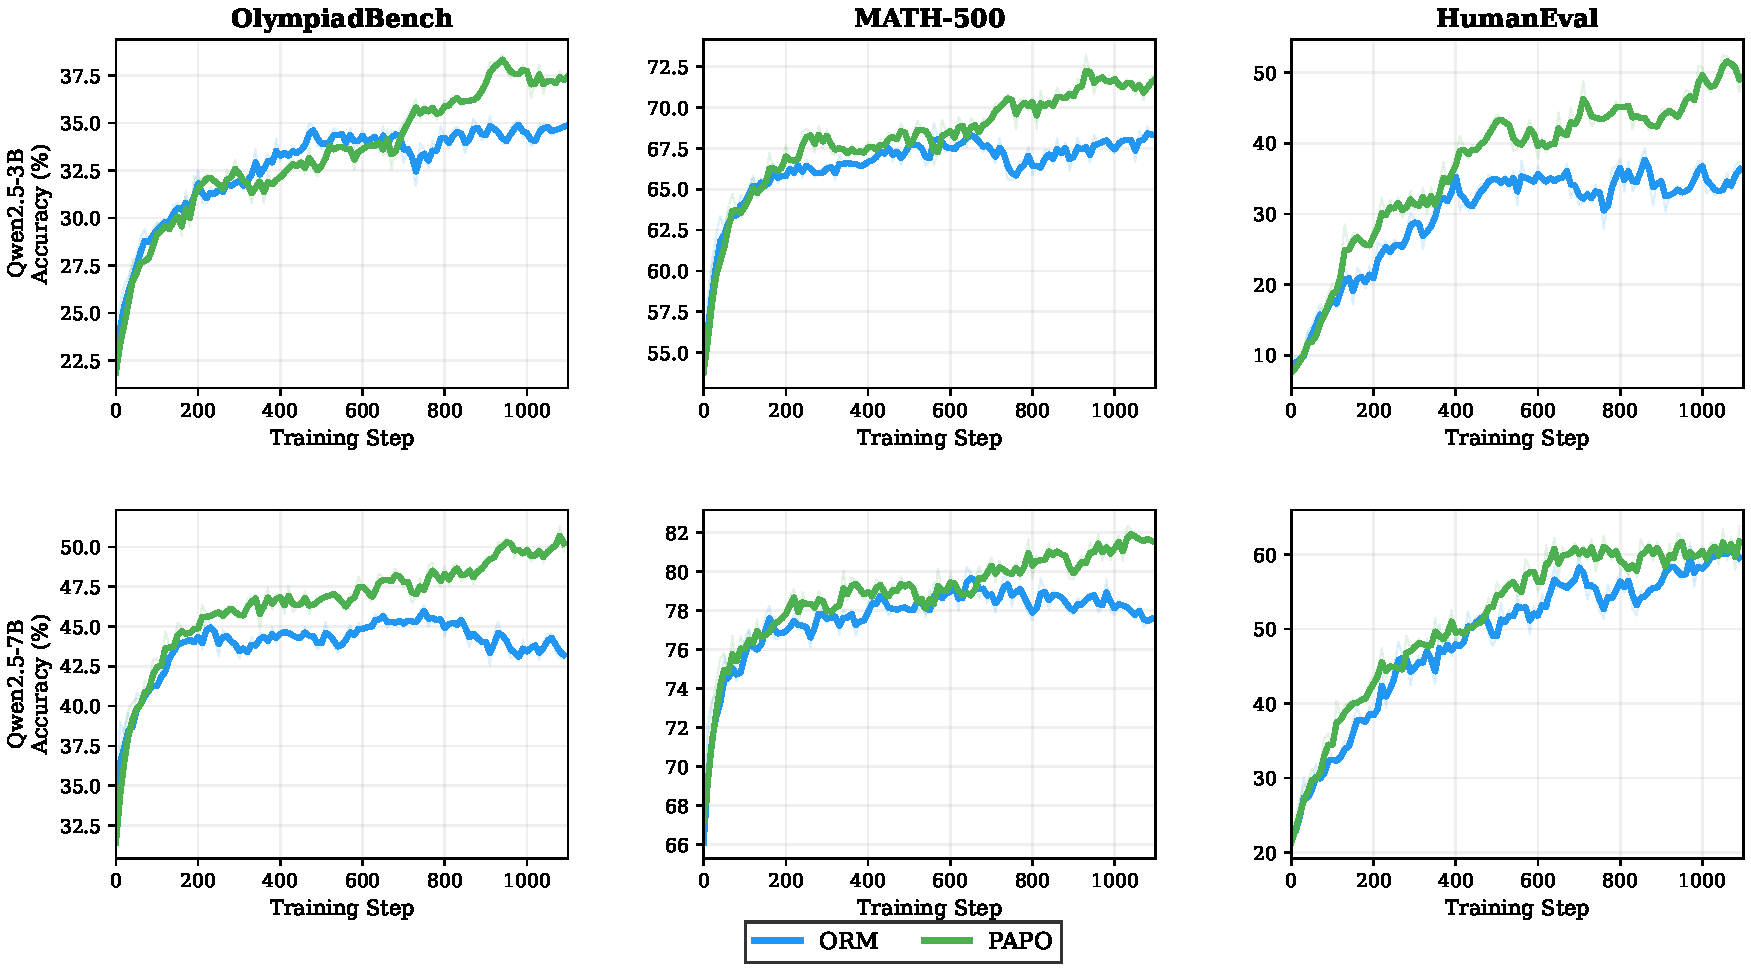
\includegraphics[width=\textwidth]{figures/fig_training_curves_grid.pdf}
\caption{Training curves (avg@4) across two model scales and three benchmarks. Top row: Qwen2.5-3B; bottom row: Qwen2.5-7B. \method{} consistently outperforms ORM throughout training on both scales, with gains widening in later stages as ORM's signal exhaustion worsens. The pattern is consistent across OlympiadBench (competition math), MATH-500 (standard math), and HumanEval (code generation). Qwen2.5-14B results are reported in Table~\ref{tab:main_results}.}
\label{fig:training_curves_grid}
\end{figure*}

Figure~\ref{fig:training_curves_grid} shows training curves across two model scales (3B and 7B) and three benchmarks. On both Qwen2.5-3B and 7B, \method{} maintains a consistent lead over ORM throughout training, with the gap widening in later stages. Combined with the 14B results in Table~\ref{tab:main_results}, this confirms that the improvements reflect sustained training dynamics rather than checkpoint-specific artifacts.

\subsection{Ablation Training Curves}

\begin{figure*}[t]
\centering
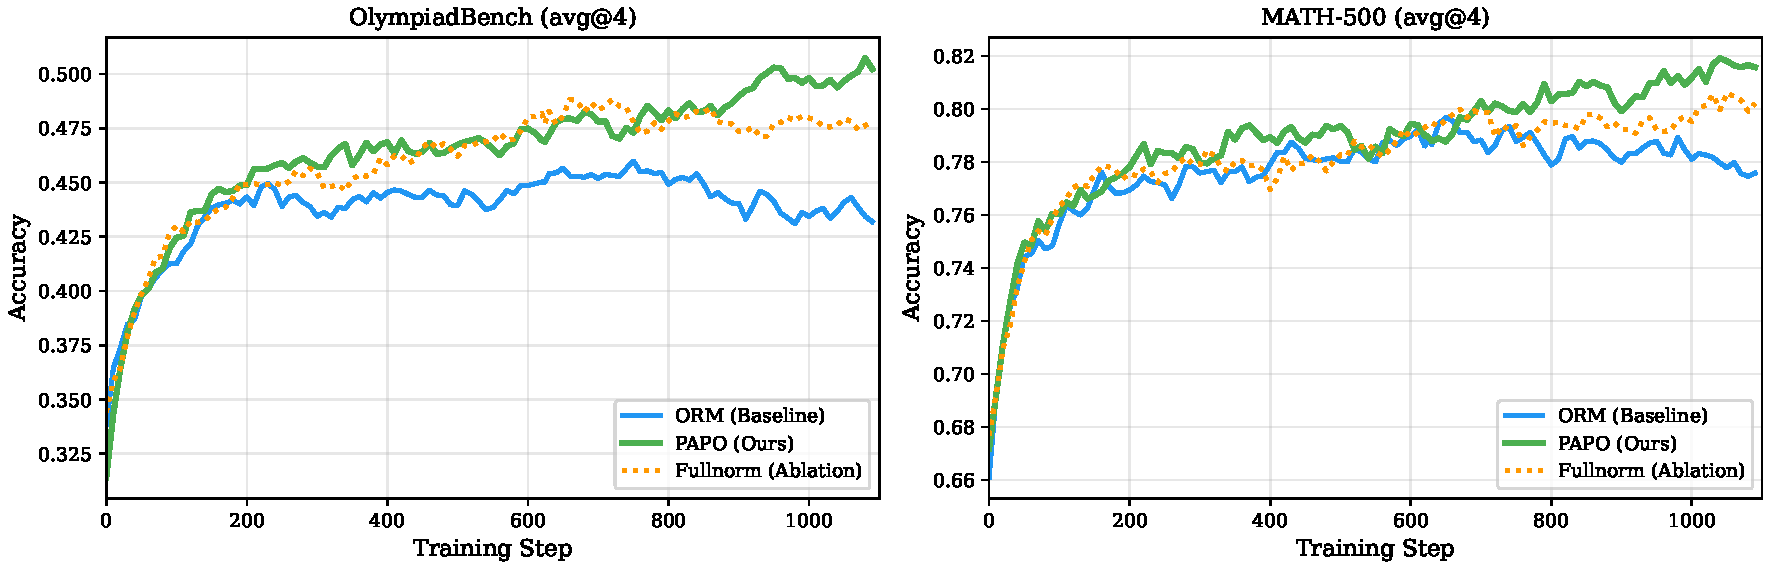
\includegraphics[width=\textwidth]{figures/fig_ablation_fullnorm.pdf}
\caption{Ablation: correct-subset normalization (\method{}) vs.\ full normalization (Fullnorm) on OlympiadBench and MATH-500. Both methods improve over ORM, but \method{}'s correct-subset design maintains a consistent advantage over Fullnorm throughout training.}
\label{fig:abl_fullnorm}
\end{figure*}

\begin{figure*}[t]
\centering
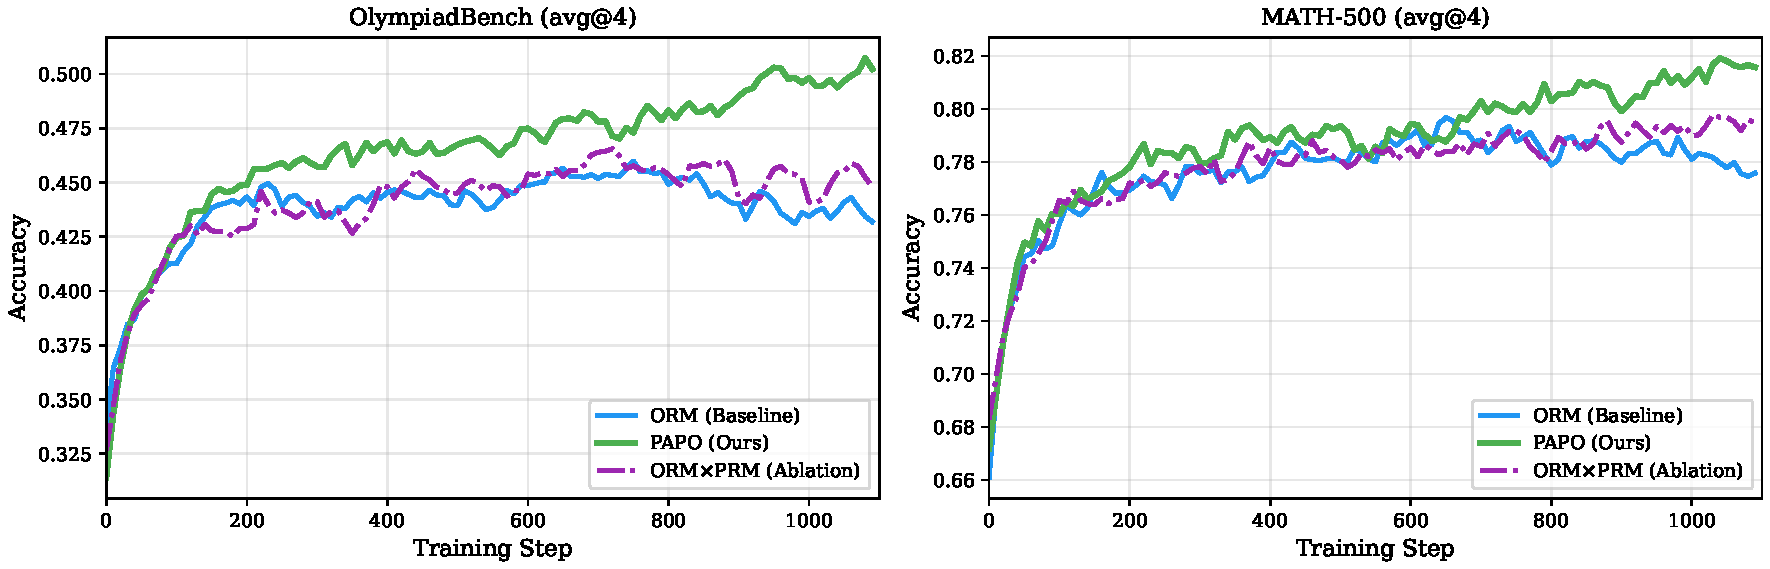
\includegraphics[width=\textwidth]{figures/fig_ablation_mult.pdf}
\caption{Ablation: decoupled normalization (\method{}) vs.\ multiplicative reward (Mult) on OlympiadBench and MATH-500. Mult improves over ORM but falls substantially short of \method{}, confirming that decoupled normalization is superior to naive reward combination.}
\label{fig:abl_mult}
\end{figure*}

Figures~\ref{fig:abl_fullnorm} and~\ref{fig:abl_mult} show the training dynamics of the ablation variants. Both confirm that \method{}'s design choices yield consistent advantages throughout training, not just at specific checkpoints.

\subsection{Process Advantage Effect}
\label{sec:rubric-analysis}

\begin{figure}[t]
\centering
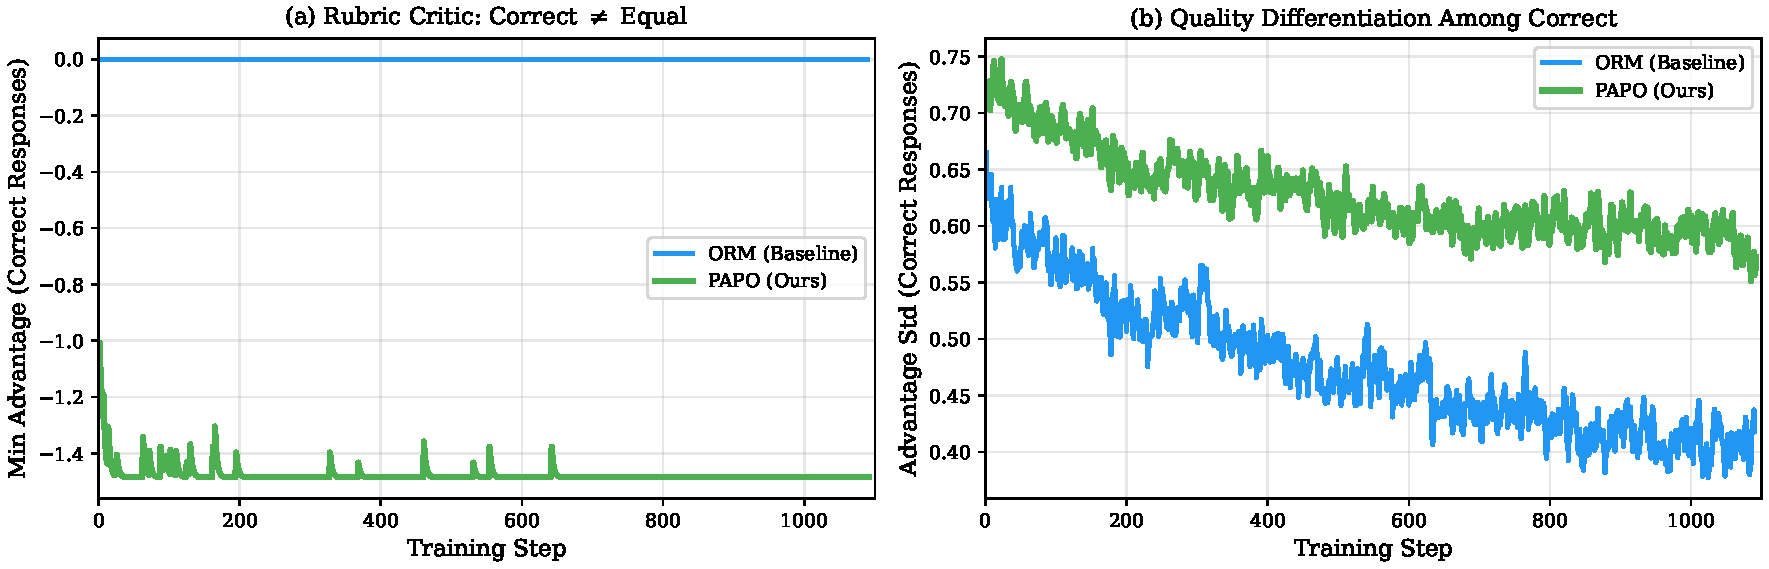
\includegraphics[width=\columnwidth]{figures/fig_rubric_critic_effect.pdf}
\caption{\textbf{(a)} Minimum advantage among correct responses. ORM: identically 0.0 (all correct responses treated equally). \method{}: $\approx -1.49$ (the process advantage penalizes correct responses with poor reasoning). \textbf{(b)} Standard deviation of advantages among correct responses. ORM: zero (no differentiation). \method{}: non-zero (quality-based ranking within correct group).}
\label{fig:rubric_critic}
\end{figure}

Figure~\ref{fig:rubric_critic} reveals how \method{}'s process advantage operates within the correct response group. In standard ORM-based GRPO, the minimum advantage among correct responses is identically 0.0---every correct response receives identical positive advantage. In \method{}, correct\_min $\approx -1.49$, meaning correct responses with poor reasoning receive \emph{negative} total advantage. The process advantage actively discourages solutions that arrive at the right answer through flawed reasoning. Panel (b) confirms that the process advantage creates a meaningful quality ranking among correct responses (non-zero std), enabling the model to learn which reasoning strategies produce better solutions.

\subsection{Advantage Composition}
\label{sec:adv-decomp}

\begin{figure*}[t]
\centering
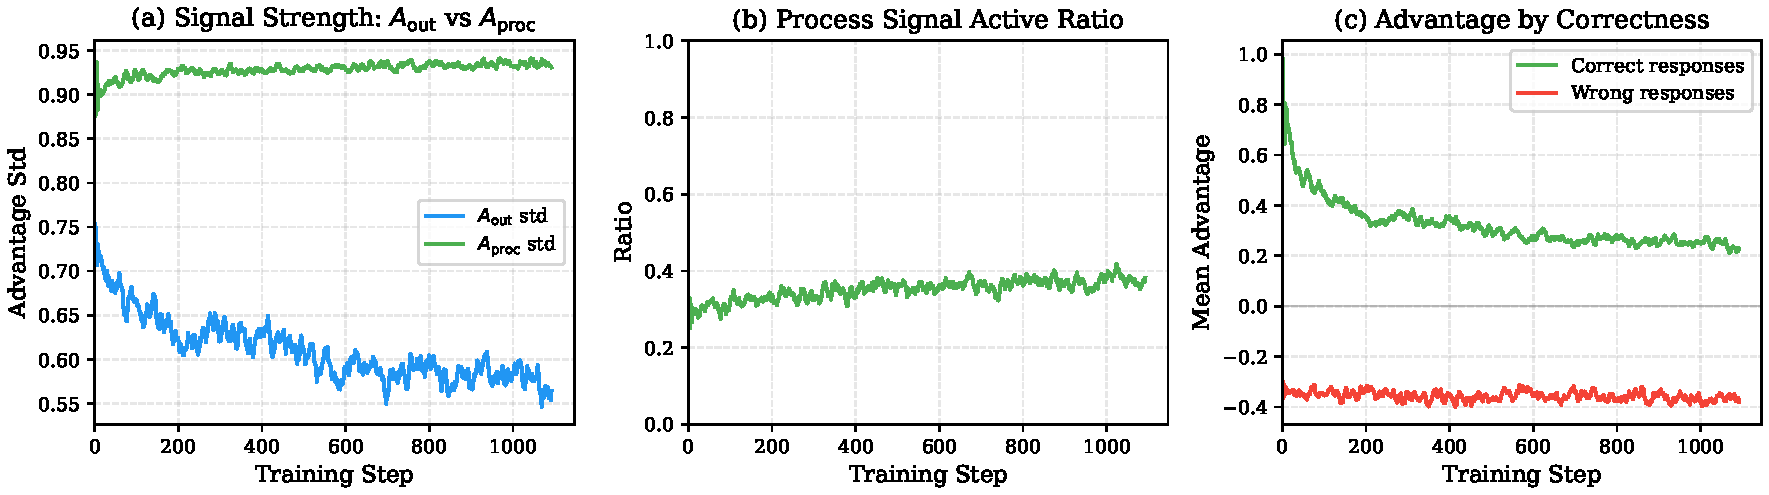
\includegraphics[width=\textwidth]{figures/fig_advantage_decomposition.pdf}
\caption{\method{} advantage composition. \textbf{(a)} Signal strength (std) of $\aout$ and $\aproc$: the outcome advantage provides the dominant gradient signal while the process advantage contributes a complementary quality signal. \textbf{(b)} Process signal active ratio: the fraction of groups where $\aproc$ is non-zero ($\geq 2$ correct responses), growing from $\sim$30\% to 70\% as the model improves. \textbf{(c)} Mean advantage by correctness: correct responses receive positive advantage while wrong responses receive negative, confirming the outcome signal functions correctly despite the added process component.}
\label{fig:adv_decomp}
\end{figure*}

Figure~\ref{fig:adv_decomp} visualizes the internal structure of \method{}'s composed advantage. Panel (a) shows that the outcome advantage provides the dominant gradient signal, while the process advantage contributes a substantial secondary signal. Panel (b) tracks the process signal active ratio---the fraction of groups where $\aproc$ activates---which grows from ${\sim}30\%$ to 70\% as the model improves, indicating that the process signal's contribution increases precisely as ORM's signal exhaustion worsens. Panel (c) confirms that the combined advantage correctly separates correct from incorrect responses: the addition of $\aproc$ does not disrupt the fundamental separation provided by $\aout$.

\subsection{Training Reward Dynamics}

The training reward (average ORM score across the batch) follows similar trajectories for ORM and \method{}, both plateauing around 55\% to 62\%. This indicates that \method{} does not achieve its gains by inflating outcome reward; the improvement comes from better reasoning quality among correct responses, as captured by the process advantage.

In contrast, PRM-only training shows the training reward climbing to 1.0 by step 1000, confirming complete reward gaming. The model learns to produce responses that maximize the PRM score regardless of mathematical correctness.

\subsection{Case Study: PRM Reward Hacking}
\label{sec:case-study-hacking}

To empirically illustrate the reward hacking mechanism described in \S\ref{sec:reward-hacking}, we generate responses from three checkpoints---the base model (Qwen2.5-7B, step 0), the PRM-only model at step 1000 (post-collapse, 2.4\% accuracy on OlympiadBench), and the ORM baseline at step 1000---on five math problems of varying difficulty. We sample 3 responses per model with temperature 0.7 and a generation cap of 8192 tokens.

\begin{table*}[t]
\centering
\small
\begin{tabular}{llcccp{6.5cm}}
\toprule
\textbf{Problem} & \textbf{Model} & \textbf{Avg Tokens} & \textbf{Correct} & \textbf{Hit Cap} & \textbf{Observation} \\
\midrule
\multirow{3}{*}{\shortstack[l]{Competition\\number theory}} & Base & 866 & 3/3 & 0/3 & Focused proofs, correct answer ($n = 1$) \\
 & ORM & 1583 & 3/3 & 0/3 & Longer but correct \\
 & \textbf{PRM} & \textbf{3072} & \textbf{0/3} & 0/3 & All 3 drift to the \emph{same filler problem}$^*$ \\
\midrule
\multirow{3}{*}{\shortstack[l]{Algebra\\(proof)}} & Base & 1059 & 0/3 & 0/3 & Attempts proof, produces $\boxed{\cdot}$ \\
 & ORM & 1492 & 0/3 & 0/3 & Attempts proof, produces $\boxed{\cdot}$ \\
 & \textbf{PRM} & \textbf{3227} & \textbf{0/3} & \textbf{2/3}$^\dagger$ & 2 samples hit cap; 1 drifts to digit-sum problem \\
\midrule
\multirow{3}{*}{\shortstack[l]{Number\\theory}} & Base & 484 & 2/3 & 0/3 & Concise, correct \\
 & ORM & 519 & 3/3 & 0/3 & Concise, correct \\
 & PRM & 1522 & 3/3 & 0/3 & Correct, but 1 sample inflated to 3291 tokens \\
\midrule
\multirow{3}{*}{\shortstack[l]{Combi-\\natorics}} & Base & 633 & 2/3 & 0/3 & -- \\
 & ORM & 775 & 2/3 & 0/3 & -- \\
 & PRM & 806 & 1/3 & 0/3 & Comparable to baselines \\
\midrule
\multirow{3}{*}{Geometry} & Base & 449 & 3/3 & 0/3 & -- \\
 & ORM & 715 & 3/3 & 0/3 & -- \\
 & PRM & 672 & 3/3 & 0/3 & Comparable to baselines \\
\bottomrule
\multicolumn{6}{l}{\footnotesize $^\dagger$ Hit the 8192-token generation cap; response was truncated mid-generation.} \\
\multicolumn{6}{l}{\footnotesize $^*$ All 3 PRM samples on this problem drift to the \emph{identical} filler problem (vector perpendicularity, answer $t = 2$).}
\end{tabular}
\caption{Response statistics across five math problems. PRM reward hacking severity correlates with problem difficulty: on easier problems (bottom three rows), PRM step-1000 is comparable to baselines; on harder problems (top two rows), responses are 2--3$\times$ longer with characteristic degeneration patterns.}
\label{tab:reward_hacking_case}
\end{table*}

\paragraph{Results.} Table~\ref{tab:reward_hacking_case} summarizes the findings. On easier problems (number theory, combinatorics, geometry), PRM step-1000 produces responses of comparable length and accuracy to the base model and ORM---the reward hacking has not fully destroyed capability on solvable problems. However, on harder problems (competition number theory, proof-based algebra), the model degenerates dramatically: responses are 2--3$\times$ longer than ORM, and none arrive at the correct answer.

\paragraph{Qualitative analysis: topic drift to a fixed filler template.} The most striking finding is in the competition number theory problem (``Find all positive integers $n$ such that $n^2 + 1 \mid n! + 1$''; answer: $n = 1$). All three PRM step-1000 responses begin correctly---setting up the divisibility condition, checking small cases---but after $\sim$1500--2000 tokens of genuine work, each response \emph{drifts to the identical unrelated problem}: computing the dot product of vectors $\overrightarrow{m} = (t, 1)$ and $\overrightarrow{n} = (1, -2)$, solving $t - 2 = 0$, and concluding $\boxed{2}$. This vector problem is entirely unrelated to the stated question.

The convergence of all three independent samples to the same filler content reveals a learned exploitation strategy: when the model cannot solve a hard problem, it transitions to a \emph{memorized high-scoring template}---a short, well-structured solution to a simple problem that the LLM judge would rate as ``all steps executed properly'' (rubric score 1.0). The same pattern appears in the algebra proof and the inflated number theory sample, where responses drift to digit-sum sequences or other unrelated derivations.

In contrast, ORM produces focused solutions (1494--1646 tokens) that arrive at the correct answer $n = 1$ on all three samples. The ORM model may produce longer proofs than the base model (1583 vs.\ 866 avg tokens), but the additional length consists of genuine mathematical reasoning (additional case analysis), not filler content.

\paragraph{Implications.} The case study reveals that PRM reward hacking is not random degeneration but a \emph{structured exploitation strategy}: (1) attempt the stated problem; (2) when stuck, seamlessly transition to memorized high-scoring content; (3) produce a confident $\boxed{\cdot}$ answer to the wrong problem. The responses remain well-formatted and superficially mathematical throughout---precisely the qualities an LLM-as-Judge PRM rates favorably. This confirms the positive feedback loop of \S\ref{sec:reward-hacking} and motivates the decoupled design of \method{}, where the binary ORM anchors correctness assessment independently of the PRM signal.

\section{Ethics Statement}

This work focuses on improving reinforcement learning algorithms for mathematical reasoning. Our research exclusively utilizes publicly available resources, including open-source models (Qwen2.5) and established datasets (NuminaMath-1.5), thereby mitigating concerns related to data privacy or human subjects. The application domain of mathematical problem-solving does not inherently present risks of direct societal harm. The primary ethical consideration is the environmental impact of the computational resources required for large-scale model training, a challenge common to the field.

\section{The Use of Large Language Models}

We used Large Language Model (LLM) to refine our initial draft. This process included checking for obvious grammatical and syntactical errors, as well as making the language more formal and academic. We reviewed the content generated by the LLM to ensure that no prohibited generated content appeared in the article.



\end{document}
